\section{Requisitos No Funcionales y Modelo de Calidad}

\subsection{Marco de Calidad: ISO/IEC 25010}

El sistema \textit{AllConnect Market} adopta el estándar \textbf{ISO/IEC 25010:2011 (SQuaRE)} como modelo de calidad de producto software. Este estándar define ocho características de calidad con sus subcaracterísticas correspondientes, proporcionando un marco sistemático para especificar, medir y evaluar la calidad del sistema.

\begin{figure}[h!]
\centering
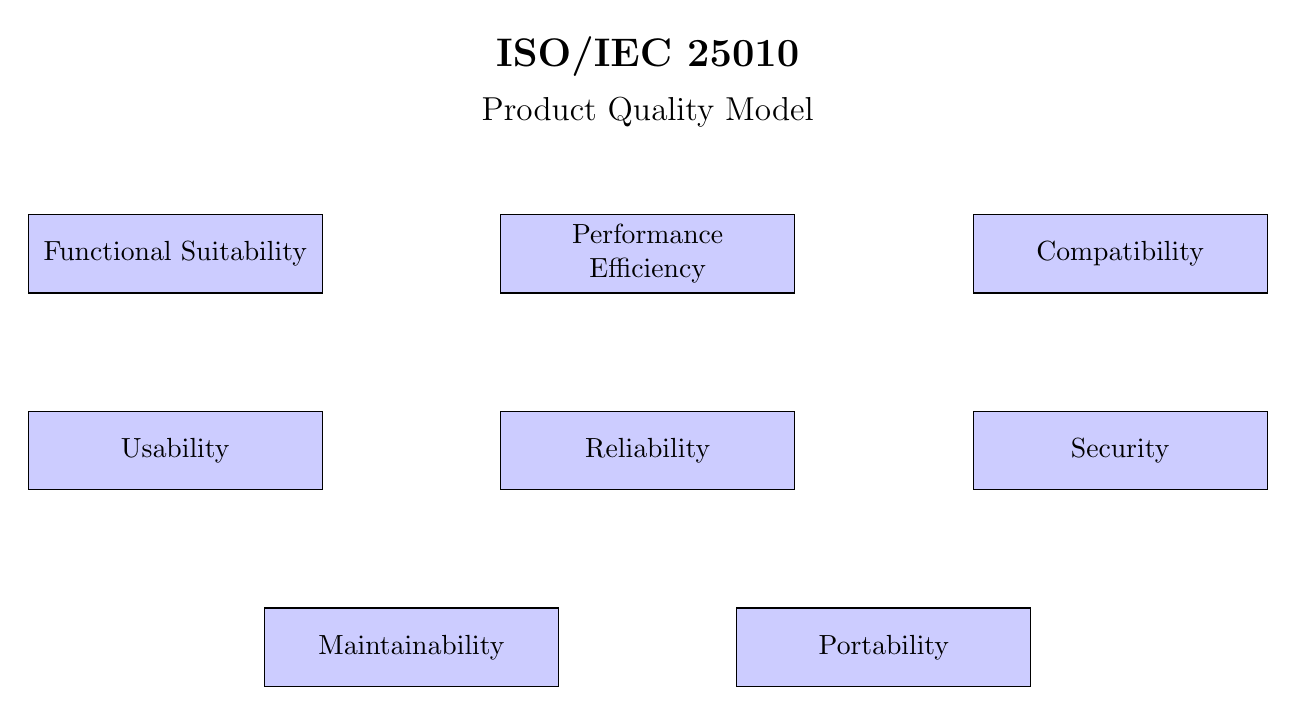
\begin{tikzpicture}[
    node distance=1.5cm,
    characteristic/.style={rectangle, draw, fill=blue!20, text width=3.5cm, align=center, minimum height=1cm}
]

% Título
\node[align=center, font=\Large\bfseries] at (0,0) {ISO/IEC 25010};
\node[align=center, font=\large] at (0,-0.7) {Product Quality Model};

% Características principales
\node[characteristic] (func) at (-6,-2.5) {Functional Suitability};
\node[characteristic] (perf) at (0,-2.5) {Performance Efficiency};
\node[characteristic] (comp) at (6,-2.5) {Compatibility};
\node[characteristic] (usab) at (-6,-5) {Usability};
\node[characteristic] (rel)  at (0,-5)  {Reliability};
\node[characteristic] (sec)  at (6,-5)  {Security};
\node[characteristic] (maint) at (-3,-7.5) {Maintainability};
\node[characteristic] (port)  at (3,-7.5)  {Portability};

\end{tikzpicture}
\caption{Modelo de calidad ISO/IEC 25010 adoptado para AllConnect Market}
\label{fig:iso25010}
\end{figure}

\subsection{Características de Calidad Priorizadas}

Las características de calidad de ISO/IEC 25010 se priorizan según su impacto en los objetivos de negocio definidos para \textit{AllConnect Market} (viabilidad económica, seguridad regulatoria y experiencia de usuario):

\begin{table}[h!]
\centering
\begin{tabular}{|l|l|p{8cm}|}
\hline
\textbf{Característica} & \textbf{Prioridad} & \textbf{Justificación de negocio} \\
\hline
Performance Efficiency & CRÍTICA & Tasa de éxito de pagos (\emph{payment success rate}) $>$ 99\% y latencias $<$ 500\,ms son requisitos de viabilidad del negocio en picos de demanda. \\
\hline
Security & CRÍTICA & Cumplimiento de buenas prácticas tipo PCI-DSS y protección de datos personales (GDPR/CCPA-like). Brechas de seguridad afectan directamente la operación y la reputación. \\
\hline
Reliability & CRÍTICA & Disponibilidad 99.9\% necesaria para alcanzar el GMV objetivo. Cada hora de \emph{downtime} implica pérdida directa de ingresos y confianza. \\
\hline
Usability & ALTA & Impacto directo en \emph{conversion rate} y \emph{cart abandonment}. Una UX competitiva es diferenciador frente a otros marketplaces. \\
\hline
Functional Suitability & ALTA & Corrección y completitud funcional validan la propuesta de valor multivertical (productos, servicios y contenidos digitales en un solo flujo). \\
\hline
Compatibility & ALTA & Interoperabilidad con APIs de proveedores y pasarelas de pago es núcleo del modelo de negocio basado en integraciones. \\
\hline
Maintainability & MEDIA & Importante para sostenibilidad a largo plazo, reducción de deuda técnica y velocidad de evolución de funcionalidades. \\
\hline
Portability & MEDIA & Despliegue \emph{cloud-native} facilita portabilidad entre nubes y flexibilidad de infraestructura, pero no condiciona el MVP. \\
\hline
\end{tabular}
\caption{Priorización de características de calidad según ISO/IEC 25010}
\label{tab:calidad-prioridad}
\end{table}

\subsection{Requisitos No Funcionales Detallados}

Los requisitos no funcionales se organizan según las características del modelo ISO/IEC 25010 y utilizan la misma metodología de priorización MoSCoW aplicada a los requisitos funcionales: MUST, SHOULD y COULD, con un \textit{rank} numérico interno de 1 a 10 para ordenar la implementación.

% ============================================================
% RNF-01: PERFORMANCE EFFICIENCY
% ============================================================

\subsubsection{RNF-01: Performance Efficiency (Eficiencia de desempeño)}

\begin{longtable}{|p{2cm}|p{1.5cm}|p{10.5cm}|}
\hline
\textbf{ID} & \textbf{Prior.} & \textbf{Requisito} \\
\hline
\endfirsthead
\hline
\textbf{ID} & \textbf{Prior.} & \textbf{Requisito} \\
\hline
\endhead

RNF-PE-001 & MUST & \textbf{Latencia de búsqueda} \newline
\textbf{Subcaracterística:} Time Behavior \newline
\textbf{Descripción:} Las búsquedas en catálogo deben retornar resultados en $<$ 500\,ms para el 95\% de las solicitudes. \newline
\textbf{Métrica:} P95 latency $<$ 500\,ms; P99 $<$ 1000\,ms. \newline
\textbf{Método de verificación:} Pruebas de carga (\emph{load testing}) con JMeter o herramienta equivalente y monitoreo APM en producción. \newline
\textbf{Justificación:} Estándar de industria. Cada 100\,ms adicionales reduce la conversión estimada en 1\%. \\
\hline

RNF-PE-002 & MUST & \textbf{Tiempo de respuesta de checkout} \newline
\textbf{Subcaracterística:} Time Behavior \newline
\textbf{Descripción:} El flujo completo de \emph{checkout} (validación + pago + confirmación) debe completarse en $<$ 5\,s para usuarios finales. \newline
\textbf{Métrica:} Tiempo \emph{end-to-end} de checkout: P95 $<$ 5\,s. \newline
\textbf{Método de verificación:} \emph{Synthetic monitoring} y \emph{Real User Monitoring} (RUM). \newline
\textbf{Justificación:} Crítico para evitar abandono de carrito y cumplir expectativas de comercio electrónico. \\
\hline

RNF-PE-003 & MUST & \textbf{Throughput de transacciones} \newline
\textbf{Subcaracterística:} Capacity \newline
\textbf{Descripción:} El sistema debe soportar, sin degradación significativa, al menos 500 transacciones de pago concurrentes. \newline
\textbf{Métrica:} TPS (\emph{Transactions Per Second}) $\geq$ 500 con latencia dentro de los umbrales definidos. \newline
\textbf{Método de verificación:} Pruebas de carga progresivas hasta 4$\times$ la capacidad objetivo. \newline
\textbf{Justificación:} Proyección para el primer año: 50\,000 órdenes/día con picos concentrados en franjas horarias. \\
\hline

RNF-PE-004 & SHOULD & \textbf{Eficiencia de almacenamiento} \newline
\textbf{Subcaracterística:} Resource Utilization \newline
\textbf{Descripción:} Las imágenes de productos deben optimizarse (por ejemplo, formato WebP) con compresión sin pérdida perceptible de calidad. \newline
\textbf{Métrica:} Reducción $\geq$ 60\% en tamaño promedio frente a imágenes originales JPEG/PNG. \newline
\textbf{Método de verificación:} Análisis de tamaño de \emph{assets} en CDN; métrica de calidad de imagen (SSIM) $>$ 0.95. \newline
\textbf{Justificación:} Reduce costos de CDN y mejora tiempos de carga en dispositivos móviles. \\
\hline

RNF-PE-005 & SHOULD & \textbf{Escalabilidad horizontal} \newline
\textbf{Subcaracterística:} Capacity \newline
\textbf{Descripción:} Los servicios \emph{backend} deben ser esencialmente \emph{stateless} para permitir \emph{auto-scaling} horizontal. \newline
\textbf{Métrica:} Tiempo de reacción de \emph{auto-scaling} $<$ 2 minutos ante incremento del 50\% en la carga. \newline
\textbf{Método de verificación:} Pruebas de \emph{spikes} de carga y \emph{chaos engineering}. \newline
\textbf{Justificación:} Preparación para eventos de alto tráfico (campañas, temporadas altas). \\
\hline

\caption{Requisitos no funcionales - Performance Efficiency}
\label{tab:rnf-performance}
\end{longtable}

% ============================================================
% RNF-02: SECURITY
% ============================================================

\subsubsection{RNF-02: Security (Seguridad)}

\begin{longtable}{|p{2cm}|p{1.5cm}|p{10.5cm}|}
\hline
\textbf{ID} & \textbf{Prior.} & \textbf{Requisito} \\
\hline
\endfirsthead
\hline
\textbf{ID} & \textbf{Prior.} & \textbf{Requisito} \\
\hline
\endhead

RNF-SEC-001 & MUST & \textbf{Procesamiento seguro de pagos} \newline
\textbf{Subcaracterística:} Confidentiality \newline
\textbf{Descripción:} El sistema debe alinearse con los requisitos de seguridad de estándares tipo PCI-DSS para procesamiento de pagos. \newline
\textbf{Criterios de aceptación:} \newline
- Tokenización inmediata de datos de tarjeta (PAN) sin almacenamiento en texto plano. \newline
- Segmentación de red para el entorno que procesa datos de tarjeta. \newline
- Registro de accesos a datos sensibles. \newline
- Auditoría periódica por tercero independiente. \newline
\textbf{Método de verificación:} Auditoría formal de seguridad y revisión de controles. \newline
\textbf{Justificación:} Requisito regulatorio y de confianza para operar con pasarelas de pago. \\
\hline

RNF-SEC-002 & MUST & \textbf{Encriptación de datos en tránsito} \newline
\textbf{Subcaracterística:} Confidentiality \newline
\textbf{Descripción:} Toda comunicación entre clientes, proveedores y servicios internos debe utilizar TLS 1.2 o superior, siendo TLS 1.3 el estándar para APIs públicas. \newline
\textbf{Criterios de aceptación:} \newline
- TLS 1.3 obligatorio para interfaces expuestas a Internet. \newline
- HSTS habilitado con \texttt{max-age} $\geq$ 1 año. \newline
- Certificados con renovación automática. \newline
\textbf{Método de verificación:} Análisis con SSL Labs (grado mínimo A) y pruebas de penetración. \newline
\textbf{Justificación:} Protección frente a ataques de tipo \emph{man-in-the-middle}. \\
\hline

RNF-SEC-003 & MUST & \textbf{Encriptación de datos en reposo} \newline
\textbf{Subcaracterística:} Confidentiality \newline
\textbf{Descripción:} Datos sensibles deben encriptarse en base de datos utilizando algoritmos robustos (por ejemplo, AES-256). \newline
\textbf{Criterios de aceptación:} \newline
- PII (correos, teléfonos, direcciones) encriptada a nivel de aplicación. \newline
- Copias de seguridad encriptadas. \newline
- Rotación de claves al menos cada 90 días. \newline
- Gestión de claves mediante HSM o KMS del proveedor cloud. \newline
\textbf{Método de verificación:} \emph{Code review} y auditoría de configuración de bases de datos. \newline
\textbf{Justificación:} Reduce impacto de posibles brechas de datos. \\
\hline

RNF-SEC-004 & MUST & \textbf{Autenticación y autorización robustas} \newline
\textbf{Subcaracterística:} Authenticity \newline
\textbf{Descripción:} Debe implementarse control de acceso basado en roles (RBAC) para todas las operaciones administrativas y de proveedor. \newline
\textbf{Criterios de aceptación:} \newline
- Uso de JWT con firma HMAC-SHA256 o RSA. \newline
- Tokens de acceso con expiración máxima de 24 horas y \emph{refresh tokens} rotados. \newline
- Roles mínimos: Cliente, Proveedor, Admin y Super Admin. \newline
- Permisos granulares por endpoint. \newline
\textbf{Método de verificación:} Pruebas de penetración y escaneos automáticos (OWASP ZAP o equivalente). \newline
\textbf{Justificación:} Prevención de accesos no autorizados y aplicación del principio de mínimo privilegio. \\
\hline

RNF-SEC-005 & MUST & \textbf{Mitigación de OWASP Top 10} \newline
\textbf{Subcaracterística:} Integrity \newline
\textbf{Descripción:} El sistema debe mitigar las vulnerabilidades más críticas recogidas en OWASP Top 10 (2021). \newline
\textbf{Criterios de aceptación:} \newline
- Inyección SQL: uso exclusivo de \emph{prepared statements} u ORMs. \newline
- XSS: sanitización de entradas y \emph{Content Security Policy}. \newline
- CSRF: tokens anti-CSRF en formularios relevantes. \newline
- Exposición de datos sensibles: registros sin PII/PCI. \newline
\textbf{Método de verificación:} SAST (por ejemplo, SonarQube), DAST (OWASP ZAP) y prueba de penetración anual. \newline
\textbf{Justificación:} Reducción de superficie de ataque y cumplimiento de buenas prácticas. \\
\hline

RNF-SEC-006 & SHOULD & \textbf{\emph{Rate limiting} y protección DDoS} \newline
\textbf{Subcaracterística:} Integrity \newline
\textbf{Descripción:} Deben existir mecanismos de \emph{rate limiting} por IP/usuario y protección ante ataques DDoS. \newline
\textbf{Criterios de aceptación:} \newline
- Límite de 100 solicitudes/minuto por IP en endpoints públicos. \newline
- Límite de 1000 solicitudes/minuto por API key de proveedor. \newline
- Uso de CDN con WAF (\emph{Web Application Firewall}). \newline
- Bloqueo automático de IPs con comportamiento malicioso. \newline
\textbf{Método de verificación:} Pruebas de carga maliciosa y \emph{stress testing}. \newline
\textbf{Justificación:} Protección de la disponibilidad y prevención de abuso de APIs. \\
\hline

RNF-SEC-007 & SHOULD & \textbf{Cumplimiento de privacidad de datos} \newline
\textbf{Subcaracterística:} Accountability \newline
\textbf{Descripción:} Implementar controles alineados con regulaciones de privacidad (por ejemplo, GDPR/CCPA). \newline
\textbf{Criterios de aceptación:} \newline
- Consentimiento explícito para procesamiento de datos (opt-in). \newline
- Portal para ejercicio de derechos tipo ARCO (acceso, rectificación, cancelación, oposición). \newline
- Política de retención: eliminación de datos tras $n$ años de inactividad (por ejemplo, 7). \newline
- Exportación de datos de usuario en formato portable (JSON/CSV). \newline
\textbf{Método de verificación:} Revisión legal y auditoría de privacidad. \newline
\textbf{Justificación:} Cumplimiento normativo y construcción de confianza con los usuarios. \\
\hline

\caption{Requisitos no funcionales - Security}
\label{tab:rnf-security}
\end{longtable}

% ============================================================
% RNF-03: RELIABILITY
% ============================================================

\subsubsection{RNF-03: Reliability (Confiabilidad)}

\begin{longtable}{|p{2cm}|p{1.5cm}|p{10.5cm}|}
\hline
\textbf{ID} & \textbf{Prior.} & \textbf{Requisito} \\
\hline
\endfirsthead
\hline
\textbf{ID} & \textbf{Prior.} & \textbf{Requisito} \\
\hline
\endhead

RNF-REL-001 & MUST & \textbf{Disponibilidad del sistema} \newline
\textbf{Subcaracterística:} Availability \newline
\textbf{Descripción:} El sistema debe mantener al menos 99.9\% de disponibilidad mensual. \newline
\textbf{Métrica:} Uptime $\geq$ 99.9\% (máximo $\approx$ 43 minutos de \emph{downtime} al mes). \newline
\textbf{Criterios de aceptación:} \newline
- SLA de 99.9\% para servicios núcleo (catálogo, carrito, pagos). \newline
- SLA de 99.5\% para servicios secundarios (notificaciones, reportes). \newline
- Ventanas de mantenimiento planificadas fuera de horas pico. \newline
\textbf{Método de verificación:} Monitoreo continuo y cálculo mensual de uptime. \newline
\textbf{Justificación:} Cada hora de caída implica pérdida directa de GMV y afecta confianza de clientes y proveedores. \\
\hline

RNF-REL-002 & MUST & \textbf{Recuperación ante fallos} \newline
\textbf{Subcaracterística:} Recoverability \newline
\textbf{Descripción:} Deben establecerse objetivos de recuperación RTO $<$ 15\,min y RPO $<$ 5\,min. \newline
\textbf{Criterios de aceptación:} \newline
- Base de datos con replicación síncrona multi-AZ. \newline
- Copias de seguridad automáticas al menos cada hora. \newline
- Plan de recuperación ante desastres documentado y probado trimestralmente. \newline
- \emph{Failover} automático de base de datos en $<$ 60\,s. \newline
\textbf{Método de verificación:} Ejercicios de \emph{disaster recovery} y pruebas de \emph{chaos engineering}. \newline
\textbf{Justificación:} Minimiza pérdida de datos y tiempo fuera de servicio. \\
\hline

RNF-REL-003 & MUST & \textbf{Tolerancia a fallos de pasarelas de pago} \newline
\textbf{Subcaracterística:} Fault Tolerance \newline
\textbf{Descripción:} El sistema debe implementar \emph{failover} automático entre pasarelas de pago cuando la principal presente degradación. \newline
\textbf{Criterios de aceptación:} \newline
- \emph{Circuit breaker} con umbral de error $>$ 10\% en ventana de 1 minuto. \newline
- Conmutación a pasarela secundaria en $<$ 5\,s. \newline
- Lógica de reintentos con \emph{backoff} exponencial para errores transitorios. \newline
- Alertas inmediatas al equipo de operaciones cuando se active el \emph{circuit breaker}. \newline
\textbf{Método de verificación:} Simulación de caída de la pasarela principal. \newline
\textbf{Justificación:} Mantener \emph{payment success rate} $>$ 99\% es requisito crítico de negocio. \\
\hline

RNF-REL-004 & SHOULD & \textbf{Degradación controlada} \newline
\textbf{Subcaracterística:} Fault Tolerance \newline
\textbf{Descripción:} Ante la caída de servicios secundarios, la plataforma debe degradar funcionalidad sin afectar el flujo principal de compra. \newline
\textbf{Criterios de aceptación:} \newline
- Falla del motor de recomendaciones $\rightarrow$ mostrar productos populares como \emph{fallback}. \newline
- Falla del servicio de \emph{reviews} $\rightarrow$ ocultar sección de reseñas. \newline
- Falla de un proveedor externo $\rightarrow$ ocultar temporalmente sus productos. \newline
- El \emph{checkout} permanece operativo mientras los servicios núcleo estén disponibles. \newline
\textbf{Método de verificación:} Pruebas con \emph{feature flags} y aislamiento de dependencias. \newline
\textbf{Justificación:} Maximizar disponibilidad percibida por el usuario y proteger la conversión. \\
\hline

RNF-REL-005 & SHOULD & \textbf{Monitoreo y observabilidad} \newline
\textbf{Subcaracterística:} Availability \newline
\textbf{Descripción:} Debe existir observabilidad completa del sistema mediante logs, métricas y trazas distribuidas. \newline
\textbf{Criterios de aceptación:} \newline
- \emph{Logging} estructurado (JSON) con \emph{correlation IDs}. \newline
- Métricas técnicas (CPU, memoria, disco) y de negocio (GMV, tasa de conversión). \newline
- \emph{Distributed tracing} con OpenTelemetry o equivalente. \newline
- Dashboards de salud por servicio con umbrales de alerta (P1--P4). \newline
\textbf{Método de verificación:} Auditoría de dashboards y simulación de incidentes. \newline
\textbf{Justificación:} Reducción del MTTD (\emph{Mean Time To Detect}) y MTTR (\emph{Mean Time To Repair}). \\
\hline

\caption{Requisitos no funcionales - Reliability}
\label{tab:rnf-reliability}
\end{longtable}

% ============================================================
% RNF-04: USABILITY
% ============================================================

\subsubsection{RNF-04: Usability (Usabilidad)}

\begin{longtable}{|p{2cm}|p{1.5cm}|p{10.5cm}|}
\hline
\textbf{ID} & \textbf{Prior.} & \textbf{Requisito} \\
\hline
\endfirsthead
\hline
\textbf{ID} & \textbf{Prior.} & \textbf{Requisito} \\
\hline
\endhead

RNF-USA-001 & MUST & \textbf{Accesibilidad WCAG 2.1 AA} \newline
\textbf{Subcaracterística:} Accessibility \newline
\textbf{Descripción:} La interfaz web debe cumplir con WCAG 2.1 nivel AA para garantizar accesibilidad. \newline
\textbf{Criterios de aceptación:} \newline
- Contraste de color mínimo 4.5:1 para texto normal. \newline
- Navegación completa por teclado (orden de tabulación lógico). \newline
- Etiquetas descriptivas en formularios. \newline
- Soporte para lectores de pantalla (atributos ARIA). \newline
- Textos alternativos en imágenes relevantes. \newline
\textbf{Método de verificación:} Auditoría con herramientas (WAVE, aXe) y pruebas con usuarios con diversidad funcional. \newline
\textbf{Justificación:} Inclusividad y cumplimiento legal en mercados regulados. \\
\hline

RNF-USA-002 & MUST & \textbf{Diseño adaptable (\emph{responsive})} \newline
\textbf{Subcaracterística:} User Interface Aesthetics \newline
\textbf{Descripción:} La interfaz debe adaptarse correctamente a móviles, tabletas y escritorio. \newline
\textbf{Criterios de aceptación:} \newline
- Puntos de quiebre: móvil ($<$ 768\,px), tableta (768--1024\,px) y escritorio ($>$ 1024\,px). \newline
- Tamaño mínimo de elementos interactivos 44$\times$44\,px en móvil. \newline
- Imágenes \emph{responsive} mediante \texttt{srcset}. \newline
\textbf{Método de verificación:} Matriz de pruebas en dispositivos y \emph{visual regression testing}. \newline
\textbf{Justificación:} Más del 60\% del tráfico objetivo se espera desde dispositivos móviles. \\
\hline

RNF-USA-003 & SHOULD & \textbf{Internacionalización (i18n)} \newline
\textbf{Subcaracterística:} Appropriateness Recognizability \newline
\textbf{Descripción:} El sistema debe soportar múltiples idiomas (español e inglés en el MVP). \newline
\textbf{Criterios de aceptación:} \newline
- Textos de interfaz extraídos a archivos de recursos de internacionalización. \newline
- Formatos de fecha, número y moneda según \emph{locale}. \newline
- Preparación de estilos para soportar idiomas de lectura derecha-izquierda (RTL). \newline
\textbf{Método de verificación:} Pruebas con diferentes \emph{locales} y revisión por hablantes nativos. \newline
\textbf{Justificación:} Facilita expansión a mercados regionales e internacionales. \\
\hline

RNF-USA-004 & SHOULD & \textbf{Facilidad de aprendizaje (\emph{learnability})} \newline
\textbf{Subcaracterística:} Learnability \newline
\textbf{Descripción:} Un usuario nuevo debe poder completar su primera compra en menos de 5 minutos sin ayuda externa. \newline
\textbf{Criterios de aceptación:} \newline
- Flujo de \emph{onboarding} con máximo 3 pasos. \newline
- Mensajes de error claros con sugerencias de corrección. \newline
- Indicador de progreso visible durante el checkout. \newline
\textbf{Método de verificación:} Pruebas de usabilidad con usuarios reales (\emph{task completion rate} $>$ 90\%). \newline
\textbf{Justificación:} Reducción de fricción y mejora de tasa de conversión. \\
\hline

RNF-USA-005 & COULD & \textbf{Retroalimentación háptica en mobile} \newline
\textbf{Subcaracterística:} User Interface Aesthetics \newline
\textbf{Descripción:} Acciones clave deben generar una vibración sutil en dispositivos móviles compatibles. \newline
\textbf{Criterios de aceptación:} \newline
- Vibración al añadir un producto al carrito. \newline
- Vibración al confirmar un pago exitoso. \newline
- Vibración de error al fallar una transacción. \newline
- Respeto de la configuración de silencio del dispositivo. \newline
\textbf{Método de verificación:} Pruebas en dispositivos iOS y Android. \newline
\textbf{Justificación:} Mejora la experiencia táctil y refuerza el feedback visual. \\
\hline

\caption{Requisitos no funcionales - Usability}
\label{tab:rnf-usability}
\end{longtable}

% ============================================================
% RNF-05: COMPATIBILITY
% ============================================================

\subsubsection{RNF-05: Compatibility (Compatibilidad)}

\begin{longtable}{|p{2cm}|p{1.5cm}|p{10.5cm}|}
\hline
\textbf{ID} & \textbf{Prior.} & \textbf{Requisito} \\
\hline
\endfirsthead
\hline
\textbf{ID} & \textbf{Prior.} & \textbf{Requisito} \\
\hline
\endhead

RNF-COMP-001 & MUST & \textbf{Interoperabilidad de APIs} \newline
\textbf{Subcaracterística:} Interoperability \newline
\textbf{Descripción:} Las APIs públicas deben seguir un estilo RESTful con documentación en OpenAPI 3.0. \newline
\textbf{Criterios de aceptación:} \newline
- Versionado explícito de API: \texttt{/api/v1}, \texttt{/api/v2}. \newline
- Documentación autogenerada (Swagger/Redoc o similar). \newline
- Validación de contratos mediante JSON Schema. \newline
- Mantenimiento de compatibilidad hacia atrás por al menos 12 meses tras publicar una nueva versión. \newline
\textbf{Método de verificación:} \emph{Contract testing} y análisis con linters de API. \newline
\textbf{Justificación:} Reduce fricción de integración con proveedores y terceros. \\
\hline

RNF-COMP-002 & MUST & \textbf{Compatibilidad entre navegadores} \newline
\textbf{Subcaracterística:} Interoperability \newline
\textbf{Descripción:} La aplicación web debe funcionar correctamente en los navegadores más utilizados por la audiencia objetivo. \newline
\textbf{Criterios de aceptación:} \newline
- Compatibilidad con versiones recientes de Chrome, Safari, Firefox y Edge. \newline
- Soporte para Chrome Android y Safari iOS en dispositivos móviles. \newline
\textbf{Método de verificación:} Pruebas cruzadas de navegador (\emph{cross-browser testing}) con BrowserStack o herramienta similar. \newline
\textbf{Justificación:} Maximiza el alcance de usuarios finales y evita dependencia de un único navegador. \\
\hline

RNF-COMP-003 & SHOULD & \textbf{Coexistencia con sistemas externos} \newline
\textbf{Subcaracterística:} Coexistence \newline
\textbf{Descripción:} El sistema debe integrarse con herramientas externas (analítica, atención al cliente) sin interferir con su funcionamiento. \newline
\textbf{Criterios de aceptación:} \newline
- Integración con Google Analytics / Tag Manager sin romper el flujo de la aplicación. \newline
- Compatibilidad con herramientas de \emph{customer service} (por ejemplo, Zendesk, Intercom). \newline
- Webhooks procesados de forma asíncrona para no bloquear el flujo de usuario. \newline
\textbf{Método de verificación:} Pruebas de integración con sistemas reales. \newline
\textbf{Justificación:} Facilita la adopción de herramientas de operación sin cambios estructurales en el sistema. \\
\hline

\caption{Requisitos no funcionales - Compatibility}
\label{tab:rnf-compatibility}
\end{longtable}

% ============================================================
% RNF-06: MAINTAINABILITY
% ============================================================

\subsubsection{RNF-06: Maintainability (Mantenibilidad)}

\begin{longtable}{|p{2cm}|p{1.5cm}|p{10.5cm}|}
\hline
\textbf{ID} & \textbf{Prior.} & \textbf{Requisito} \\
\hline
\endfirsthead
\hline
\textbf{ID} & \textbf{Prior.} & \textbf{Requisito} \\
\hline
\endhead

RNF-MAIN-001 & SHOULD & \textbf{Modularidad de código} \newline
\textbf{Subcaracterística:} Modularity \newline
\textbf{Descripción:} La arquitectura debe seguir principios de microservicios con bajo acoplamiento entre componentes. \newline
\textbf{Criterios de aceptación:} \newline
- Servicios independientes alineados con \emph{bounded contexts} de negocio. \newline
- Comunicación entre servicios mediante APIs/eventos, sin acceso directo cruzado a bases de datos. \newline
- Despliegue independiente de cada servicio. \newline
\textbf{Método de verificación:} Análisis de dependencias y \emph{architectural fitness functions}. \newline
\textbf{Justificación:} Facilita la evolución del sistema y el trabajo de equipos autónomos. \\
\hline

RNF-MAIN-002 & SHOULD & \textbf{Testabilidad} \newline
\textbf{Subcaracterística:} Testability \newline
\textbf{Descripción:} El código debe contar con una cobertura de pruebas mínima del 80\% (unitarias + integración). \newline
\textbf{Criterios de aceptación:} \newline
- Pruebas unitarias con al menos 80\% de cobertura de código. \newline
- Pruebas de integración para todos los endpoints públicos. \newline
- Pruebas de contrato para integraciones con proveedores. \newline
- Pruebas E2E para flujos críticos (registro, login, checkout, pago). \newline
\textbf{Método de verificación:} Informes de cobertura en la \emph{pipeline} de CI/CD. \newline
\textbf{Justificación:} Aumenta la confianza en los cambios y reduce el riesgo de regresiones. \\
\hline

RNF-MAIN-003 & SHOULD & \textbf{Analizabilidad de código} \newline
\textbf{Subcaracterística:} Analyzability \newline
\textbf{Descripción:} El código debe cumplir estándares de calidad medibles mediante análisis estático. \newline
\textbf{Criterios de aceptación:} \newline
- \emph{Quality gate} en SonarQube con calificación de mantenibilidad A. \newline
- Complejidad ciclomatica $<$ 10 por función. \newline
- Duplicación de código $<$ 3\%. \newline
\textbf{Método de verificación:} Análisis estático en la CI/CD. \newline
\textbf{Justificación:} Facilita depuración, mantenimiento y reduce deuda técnica. \\
\hline

RNF-MAIN-004 & COULD & \textbf{Documentación técnica estructurada} \newline
\textbf{Subcaracterística:} Analyzability \newline
\textbf{Descripción:} Las decisiones arquitectónicas relevantes deben documentarse mediante \emph{Architecture Decision Records} (ADR). \newline
\textbf{Criterios de aceptación:} \newline
- ADRs en formato Markdown versionados en el repositorio. \newline
- Un \texttt{README.md} por servicio con propósito, configuración y despliegue. \newline
- Diagramas C4 actualizados para vistas arquitectónicas clave. \newline
\textbf{Método de verificación:} Revisión de documentación durante los \emph{code reviews}. \newline
\textbf{Justificación:} Facilita el \emph{onboarding} de nuevos desarrolladores y la preservación del conocimiento. \\
\hline

\caption{Requisitos no funcionales - Maintainability}
\label{tab:rnf-maintainability}
\end{longtable}

% ============================================================
% RESUMEN RNF
% ============================================================

\subsection{Resumen de Priorización de Requisitos No Funcionales}

La tabla \ref{tab:resumen-rnf} sintetiza la priorización de los requisitos no funcionales definidos en las secciones anteriores (tablas \ref{tab:rnf-performance}--\ref{tab:rnf-maintainability}). Cada RNF fue clasificado según la escala MoSCoW, tomando en cuenta su impacto en la viabilidad del negocio, cumplimiento regulatorio, riesgo operativo y complejidad técnica.

\begin{table}[h!]
\centering
\begin{tabular}{|l|c|c|c|c|}
\hline
\textbf{Característica ISO/IEC 25010} & \textbf{MUST} & \textbf{SHOULD} & \textbf{COULD} & \textbf{Total} \\
\hline
Performance Efficiency & 3 & 2 & 0 & 5 \\
Security               & 5 & 2 & 0 & 7 \\
Reliability            & 3 & 2 & 0 & 5 \\
Usability              & 2 & 2 & 1 & 5 \\
Compatibility          & 2 & 1 & 0 & 3 \\
Maintainability        & 0 & 3 & 1 & 4 \\
\hline
\textbf{TOTAL}         & \textbf{15} & \textbf{12} & \textbf{2} & \textbf{29} \\
\hline
\end{tabular}
\caption{Distribución de prioridades de requisitos no funcionales por característica de calidad}
\label{tab:resumen-rnf}
\end{table}

\subsubsection*{Lectura de la tabla}
\begin{itemize}
    \item \textbf{15 RNF MUST (52\%)}: constituyen el \emph{mínimo nivel de calidad} requerido para que el MVP pueda operar de manera segura, estable y conforme a regulación.
    \item \textbf{12 RNF SHOULD (41\%)}: fortalecen escalabilidad, operación continua y experiencia de usuario; forman parte de la evolución inmediata post-MVP.
    \item \textbf{2 RNF COULD (7\%)}: mejoras de refinamiento que aportan diferenciación sin afectar la operación central.
\end{itemize}

\subsubsection*{Análisis por foco de calidad}

\begin{enumerate}
    \item \textbf{Calidad esencial para operación y cumplimiento regulatorio} \\
    Las características \textit{Security}, \textit{Performance Efficiency} y \textit{Reliability} concentran \textbf{11 de los 15 MUST}:
    \begin{itemize}
        \item \textbf{Security (5 MUST)}: incluye PCI-DSS, cifrado, mitigación OWASP Top 10 y control de acceso. Sin estos requisitos, el sistema no puede procesar pagos ni manejar datos sensibles.
        \item \textbf{Performance Efficiency (3 MUST)}: asegura tiempos de respuesta bajos en búsqueda y checkout, impactando directamente el conversion rate.
        \item \textbf{Reliability (3 MUST)}: garantiza disponibilidad 99.9\%, recuperación ante fallos y continuidad del flujo de pagos.
    \end{itemize}
    Estos requisitos definen el \textbf{piso técnico y regulatorio} indispensable para lanzar el MVP.

    \item \textbf{Sostenibilidad, experiencia y ecosistema técnico} \\
    Las características \textit{Usability}, \textit{Compatibility} y \textit{Maintainability} contienen en su mayoría RNF \textbf{SHOULD} y \textbf{COULD}:
    \begin{itemize}
        \item \textbf{Usability}: accesibilidad WCAG 2.1 y responsive design son MUST; mejoras como onboarding guiado o feedback háptico se abordan como SHOULD/COULD.
        \item \textbf{Compatibility}: interoperabilidad API y compatibilidad cross-browser son MUST; integraciones externas se tratan como SHOULD.
        \item \textbf{Maintainability}: modularidad, testabilidad y calidad de código son SHOULD; documentación arquitectónica (ADRs) es COULD. No bloquean el MVP, pero impactan la velocidad de evolución.
    \end{itemize}
    Este conjunto estructura la \textbf{madurez técnica y operativa} del sistema después del lanzamiento inicial.

    \item \textbf{Enfoque de iteraciones desde la perspectiva de calidad}
    \begin{itemize}
        \item \textbf{Iteración 1 (MVP – salida a producción):} implementación de todos los RNF \textbf{MUST}, garantizando seguridad transaccional, disponibilidad, interoperabilidad básica y UX mínima.
        \item \textbf{Iteración 2 (Escalado y eficiencia operativa):} ejecución de los RNF \textbf{SHOULD}, priorizando maintainability (tests, análisis estático), observabilidad, escalabilidad horizontal, i18n y mejoras de usabilidad.
        \item \textbf{Iteración 3+ (Diferenciación y refinamiento):} implementación de RNF \textbf{COULD}, como feedback háptico o documentación arquitectónica avanzada.
    \end{itemize}
\end{enumerate}
